\documentclass{article}
\usepackage{graphicx} % Required for inserting images
\usepackage{hyperref}
\usepackage{caption} % For custom captions
\usepackage{amsmath}
\usepackage{multicol}

\title{Theoretical Mechanics: Week Homework 8}
\author{Ekaterina Mozhegova}
\date{March 19, 2024}

\begin{document}

\maketitle

\section{Link}
\href{https://github.com/illusoryTwin/Theoretical_mechanics/tree/master/hw7}{Link to the github repository containing all the materials}

\section{Task 1}

\subsection{Task Description}

A mechanical system under the gravity force moves from the rest. Define the velocity of object $A$ if it travels distance $s$ from the rest. The masses of the non-deformable ropes are ignored. Neglect the masses of links $FK,\ KC$ and the piston $K$.

The task is to:
\begin{enumerate}
    \item make a plot $v_A(s)$;
    \item What will change if we omit the last sentence (Neglect ...). (Explain it and show on equations). Why Yablonskii made these constraints?
\end{enumerate}

Needed variables:\\
$m_A=1,\ m_B=3,\ m_D=20$ (kg);\\
$R_B=20,\ R_D=20,\ i_{Bx}= 18$ (cm), $i_{Bx}$ - radii of gyration of the body;\\
$\psi = 0.6$ (cm), where $\psi$ is rolling friction.
   
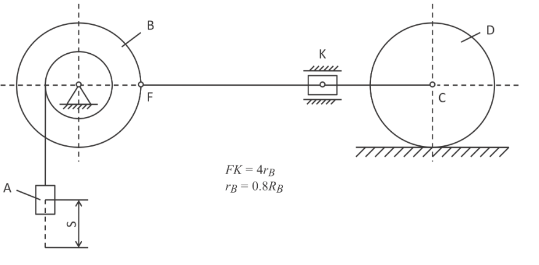
\includegraphics[scale=0.5]{hw8_task1.png}

\subsection{Task Explanation}

\subsubsection{Neglect masses}

\textbf{Research object:} A system of a body A, wheels B, wheel D\\
\textbf{Motion:} A - plane motion, B - rotational motion, D - rotational and plane motions\\
\textbf{Force analysis:} $F_\text{fr} = \psi N$, 
% F_\text{grav} = m_2 g s$\\
\textbf{Solution:}

\[T = A \text{, where } T = \sum T_i, A = \sum A_i\]


\[
T = T_A + T_{\text{B\_rot}} + T_{\text{D\_rot}} + T_D
\]

\[
h = \sin\left(\frac{s \cdot 180}{\pi \cdot r_b}\right) \cdot R_b
\]

\[
T_A = \frac{m_a \cdot \text{dot\_s}^2}{2}
\]

% \[
% T_{\text{B\_rot}} = \frac{\left(\frac{\text{\dot{s}}}{r}\right)^2 \times J_b}{2}
% \]

% \[
% T_{\text{D\_rot}} = \frac{m_d \times \left(\frac{25}{16} \times \text{\dot{s}}^2 \times \left(FK^2 - h^2\right)\right)}{4}
% \]

% \[
% T_D = \frac{m_d \times \left(\frac{25}{16} \times \text{dot\_s}^2 \times \left(FK^2 - h^2\right)\right)}{2}
% \]





\begin{align*}
    y_d &= l \sin(\alpha) & \dot{y}_d &= l \dot{\alpha} \cos(\alpha) \\
    x_d &= l \cos(\alpha) & \dot{x}_d &= -l \dot{\alpha} \sin(\alpha)
\end{align*}


\[ \dot \alpha = \omega = \dot \alpha = \dfrac{v_b}{2l \cos \alpha}\]

\[V_d^2 = (l \cos(\alpha) \dot{\alpha})^2 + (-l \sin(\alpha) \dot{\alpha})^2 = l^2 (\dot{\alpha})^2 = l \omega^2\]

\[V_d^2 = l^2 \omega^2 = l^2 \cdot \frac{v_b^2}{4l^2 \cos^2(\alpha)}\]

\[T_\text{rot} = \dfrac{J \omega^2}{2} = \dfrac{m \rho^2 \omega^2}{2} = \dfrac{m \rho^2}{2} \dfrac{V_b^2}{4l^2 \cos(\alpha)^2}\]

\[T_1 = T + T_{\text{rot}} = \frac{mV_d^2}{2} + \frac{J \omega^2}{2} = \frac{m V_b^2}{2 \cdot 4 \cos^2(\alpha)} + \frac{m \rho^2 V_b^2}{2 \cdot 4l^2 \cos^2(\alpha)}\]

\[T_\text{tot} = 2T_1 = 2 (\frac{m V_b^2}{2 \cdot 4 \cos^2(\alpha)} + \frac{m \rho^2 V_b^2}{2 \cdot 4l^2 \cos^2(\alpha)}) = \frac{m V_b^2}{4 \cos^2(\alpha)} + \frac{m \rho^2 V_b^2}{4l^2 \cos^2(\alpha)}\]

\textbf{Work:}

2 gravitational forces do job (of a rod 1 and of a rod 2).

Due to the symmetry:

\[A_\text{tot} = 2A_G = 2 mg \Delta h = 2mg ( \frac{h}{2} - l \sin(\alpha))\]
 
\begin{enumerate}
  \item When B hits the floor, $\alpha = 0$, so $A_\text{tot} = 2 m g \frac{h}{2} = mgh$
    \begin{center}
      For $\alpha = 0$ we have: $\cos(\alpha) = 1$, $\sin(\alpha) = 0$.
    \end{center}
    \[ \frac{m V_b^2}{4 \cos^2(\alpha)} + \frac{m \rho^2 V_b^2}{4l^2 \cos^2(\alpha)} = mgh\]
    \[ \frac{m V_b^2}{4 \cdot 1} (1 + \frac{\rho^2}{l^2}) = mgh\]
    \[ \frac{V_b^2}{4} (\frac{l^2 + \rho^2}{l^2}) = gh\]
    \[ V_b = \sqrt{\dfrac{4l^2gh}{l^2 + \rho^2}} = 2l \sqrt{\dfrac{gh}{l^2 + \rho^2}}\]
    \[ \text{So, } V_b = 2l \sqrt{\dfrac{gh}{l^2 + \rho^2}}\]


  \item When B  is at the distance $ \frac{1}{2} h$ from the floor. 
    \[\sin(\alpha) = \dfrac{\frac{h}{2}}{2l} = \dfrac{h}{4l}\]
    \[\text{Thus, } \cos(\alpha)^2 = 1 - \sin(\alpha)^2 = \dfrac{16l^2 - h^2}{16l^2}\]
    \[ \frac{m V_b^2}{4 \cdot \dfrac{16l^2 - h^2}{16l^2}} (\dfrac{\rho^2 + l^2}{l^2}) = 2mg(\frac{h}{2} - l \sin(\alpha))\]
    \[ \frac{m V_b^2}{\dfrac{16l^2 - h^2}{4l^2}} (\dfrac{\rho^2 + l^2}{l^2}) = 2mg(\frac{h}{2} - l \frac{h}{4l})\]
    \[ \frac{4 mV_b^2 (l^2+\rho^2)}{16l^2 - h^2} = \dfrac{mgh}{2}\]
    \[ \frac{4 V_b^2 (l^2+\rho^2)}{16l^2 - h^2} = \dfrac{gh}{2}\]
    \[ V_b = \sqrt{\dfrac{gh(16l^2-h^2)}{2 \cdot 4(l^2 + \rho^2)}} = \dfrac{1}{2} \sqrt{\dfrac{gh(16l^2 - h^2)}{2(l^2 + \rho^2)}}\]
    \[ \text{So, } V_b = \dfrac{1}{2} \sqrt{\dfrac{gh(16l^2 - h^2)}{2(l^2 + \rho^2)}}\]
\end{enumerate}

\textbf{Answer:}
\begin{enumerate}
  \item \[V_b = 2l \sqrt{\dfrac{gh}{l^2 + \rho^2}}\]
  \item \[V_b = \dfrac{1}{2} \sqrt{\dfrac{gh(16l^2 - h^2)}{2(l^2 + \rho^2)}}\]
\end{enumerate}

\section{Task 2}

\subsection{Task Description}

You have a a cart pole. Body $1$ is a slider, mass $m_1$, it moves without friction.

$AB$ is a massless rod with length $l$. Body $2$ with mass $m_2$ is connected to $AB$ in point $B$.
\medskip

It's a 2 DoF system. You should take $x$ and $\phi$ as a repFresentation of this system. The origin of each coordinate should be the same as on the picture.
\medskip

Initial conditions:
\begin{enumerate}
  \item $x = 0,\ \phi = 10^\circ,\ \dot{x} = 0,\ \dot{\phi} = 0,\ t=0$;
  \item $x = 0.5,\ \phi = 45^\circ,\ \dot{x} = 0,\ \dot{\phi} = 0,\ t=0$;
  \item $x = 0.5,\ \phi = -135^\circ,\ \dot{x} = 0,\ \dot{\phi} = 0,\ t=0$;
\end{enumerate}
Parameters: $m_1 = 5\ kg,\ m_2 = 1\ kg,\ l = 1\ m$.

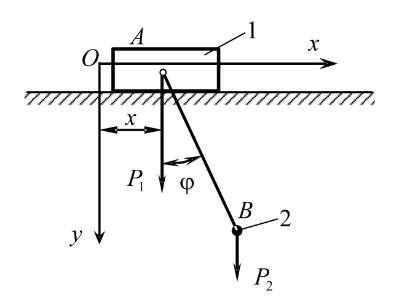
\includegraphics[scale=0.5]{hw8_task2.png}

\subsection{Task Explanation}

\textbf{Research object:} A system of 2 bodies: cart and pole\\
\textbf{Motion:} A cart - plane motion, pole - rotational motion\\
\textbf{Force analysis:} $G_1 = m_1 g$, $G_2 = m_2 g, T, N$\\
\textbf{Solution:}

\begin{align*}
  x_2 &= x + l \sin(\phi) & \dot{x_2} &= \dot{x} + l \dot{\phi} \cos(\phi) \\
  y_2 &= -l \cos(\phi) & \dot{y_2} &= l \dot{\phi} \sin(\phi)
\end{align*}

Let's define the kinetic energy (T):

\[T = \frac{1}{2} m \dot{x}^2 + \frac{1}{2} m_2 (\dot{x}^2 + \dot{y}^2) = \frac{1}{2} m_1 \dot{x}^2 + \frac{1}{2} m_2 (\dot{x}^2 + 2 \dot{x} l \dot{\phi} \cos{\phi} + l^2 \dot{\phi}^2 \cos^2{\phi} + l^2 \dot{\phi}^2 \sin^2{\phi})\]

\[T = \frac{1}{2} (m_1+m_2) \dot{x}^2  + m_2 \dot{x} l \dot{\phi} \cos{\phi} + \frac{1}{2} m_2 l^2 \dot{\phi}^2\]

Define the potential energy (V):

\[V = m_2 g y_2 = -m_2 g l \cos(\phi)\]

Define the Lagrangian (L) as the difference between kinetic and potential energy.
\[L = T - V = \frac{1}{2} (m_1+m_2) \dot{x}^2  + m_2 \dot{x} l \dot{\phi} \cos{\phi} + \frac{1}{2} m_2 l^2 \dot{\phi}^2 + m_2 g l \cos(\phi)\]

Calculate partial derivatives of the Lagrangian with respect to generalized coordinates and velocities.
\[ \frac{\partial L}{\partial \dot{x}} = (m_1+m_2) \dot{x} + m_2 l \dot{\phi} \cos(\phi)\]

\[ \frac{\partial L}{\partial x} = 0\]

\[ \frac{\partial L}{\partial \dot{\phi}} = m_2 \dot x l \cos(\phi) + m_2 l^2 \dot \phi\]

\[ \frac{\partial L}{\partial \phi} = -m_2 \dot x l \dot \phi \sin(\phi) - m_2 g l \sin(\phi)\]

Apply the Euler-Lagrange equations to find the equations of motion.

\[\frac{d}{dt} \left( \frac{\partial L}{\partial \dot{\phi}} \right) = m_2 \dot{x} l \cos(\phi) - \dot{\phi} m_2 \dot{x} l \sin(\phi) + m_2 l^2 \dot{\phi}
\] 

\[\frac{d}{dt} \left( \frac{\partial L}{\partial \dot{x}} \right) = (m_1+m_2) \ddot x + m_2 l \ddot \phi \cos(\phi) - m_2 g l \sin(\phi)\]

\[\frac{d}{dt} \left( \frac{\partial L}{\partial \dot{\phi}} \right) - \frac{\partial L}{\partial \phi} = 0\]

\[\frac{d}{dt} \left( \frac{\partial L}{\partial \dot{x}} \right) - \frac{\partial L}{\partial x} = 0\]

Solving the system computationally will provide us with the results below.


\subsection{Plots}
\subsection{Simulation}
\subsection{Discussion}
As we can see, both Newton-Euler and Lagrange-Euler methods provide us with the same solutions.
\end{document}